\section{oosalizer/output.c-Dateireferenz}
\label{output_8c}\index{oosalizer/output.c@{oosalizer/output.c}}
{\tt \#include $<$time.h$>$}\par
{\tt \#include $<$stdio.h$>$}\par
{\tt \#include $<$stdlib.h$>$}\par
{\tt \#include $<$string.h$>$}\par
{\tt \#include $<$unistd.h$>$}\par
{\tt \#include $<$ctype.h$>$}\par
{\tt \#include $<$sys/utsname.h$>$}\par
{\tt \#include $<$sys/times.h$>$}\par
{\tt \#include $<$sys/types.h$>$}\par
{\tt \#include \char`\"{}webalizer.h\char`\"{}}\par
{\tt \#include \char`\"{}lang.h\char`\"{}}\par
{\tt \#include \char`\"{}hashtab.h\char`\"{}}\par
{\tt \#include \char`\"{}preserve.h\char`\"{}}\par
{\tt \#include \char`\"{}linklist.h\char`\"{}}\par
{\tt \#include \char`\"{}graphs.h\char`\"{}}\par
{\tt \#include \char`\"{}output.h\char`\"{}}\par


Include-Abh\"{a}ngigkeitsdiagramm f\"{u}r output.c:\begin{figure}[H]
\begin{center}
\leavevmode
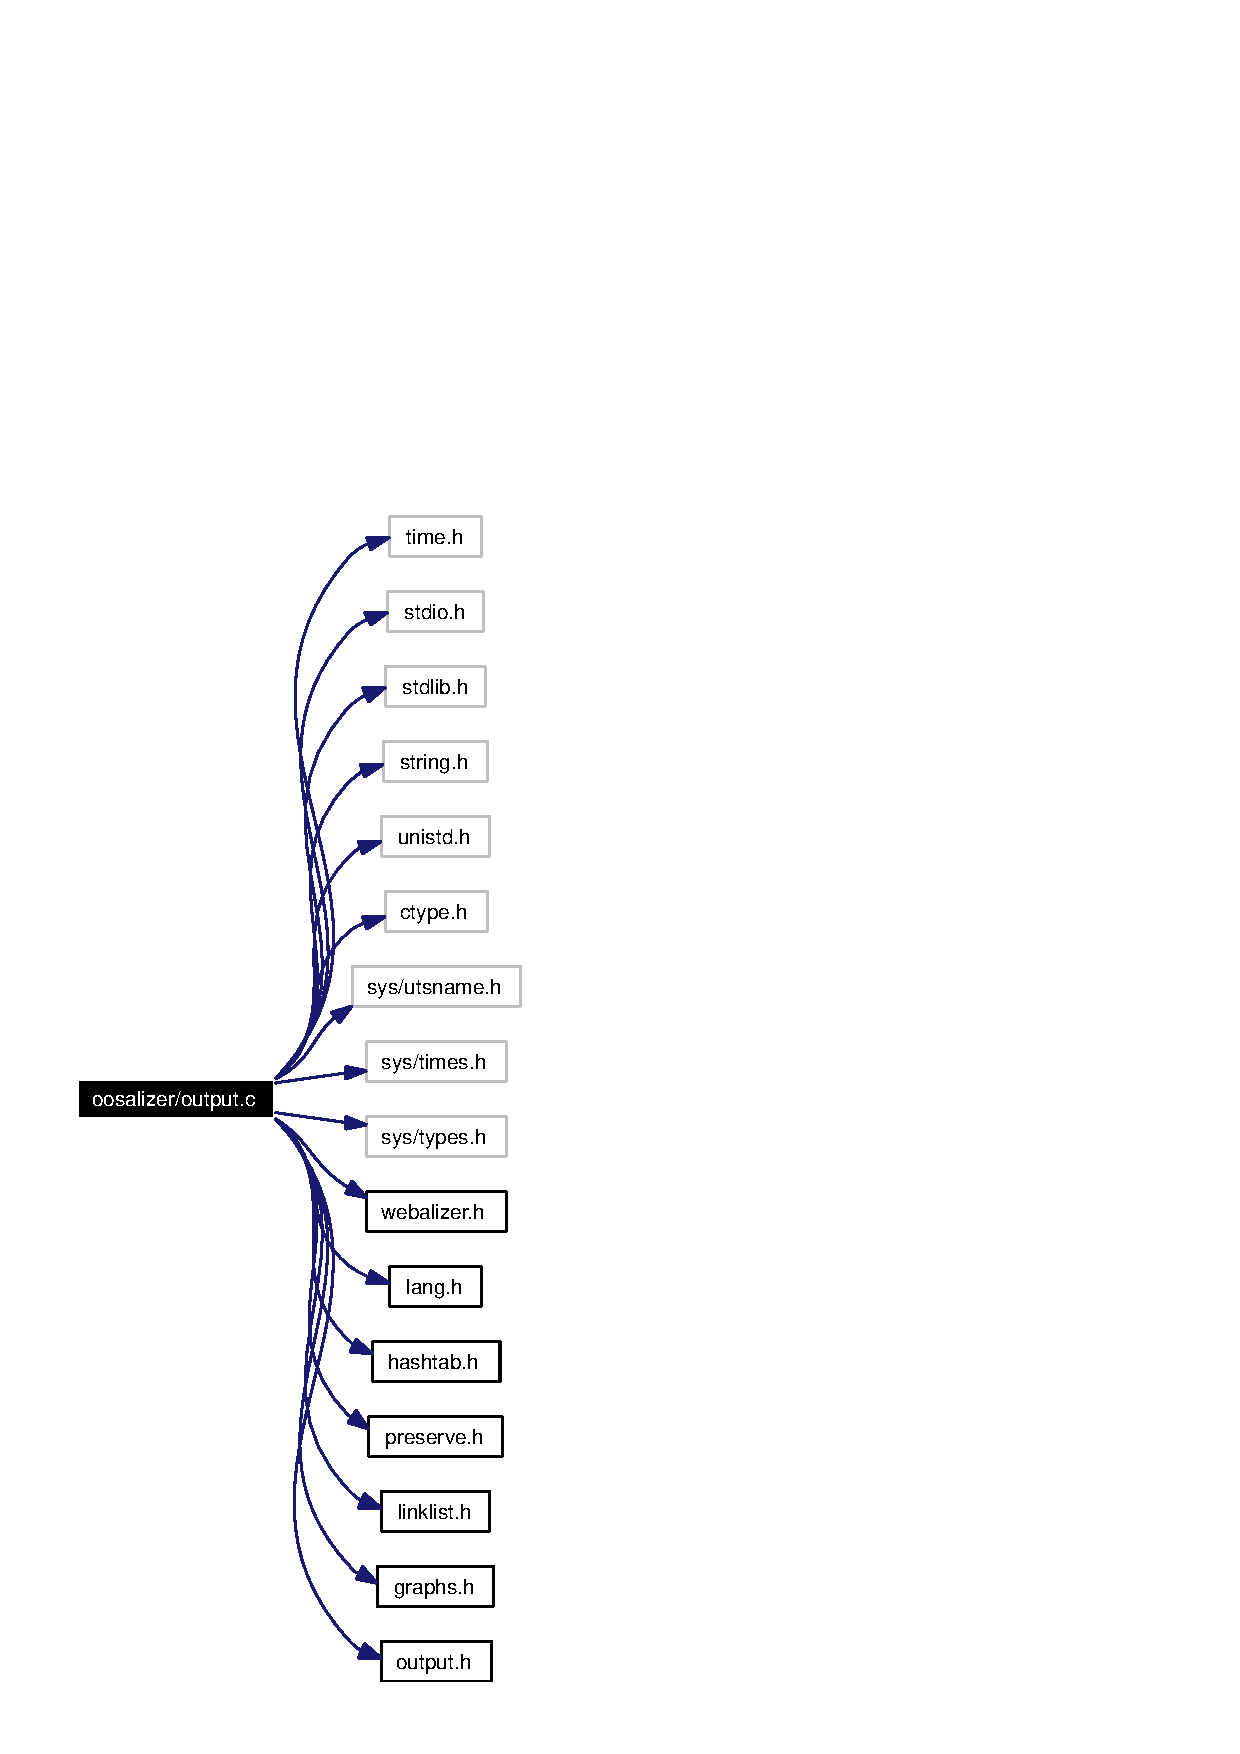
\includegraphics[width=125pt]{output_8c__incl}
\end{center}
\end{figure}
\subsection*{Makrodefinitionen}
\begin{CompactItemize}
\item 
\#define {\bf CLK\_\-TCK}~\_\-SC\_\-CLK\_\-TCK
\item 
\#define {\bf WHITE}~\char`\"{}\#FFFFFF\char`\"{}
\item 
\#define {\bf BLACK}~\char`\"{}\#000000\char`\"{}
\item 
\#define {\bf RED}~\char`\"{}\#FF0000\char`\"{}
\item 
\#define {\bf ORANGE}~\char`\"{}\#FF8000\char`\"{}
\item 
\#define {\bf LTBLUE}~\char`\"{}\#0080FF\char`\"{}
\item 
\#define {\bf BLUE}~\char`\"{}\#0000FF\char`\"{}
\item 
\#define {\bf GREEN}~\char`\"{}\#00FF00\char`\"{}
\item 
\#define {\bf DKGREEN}~\char`\"{}\#008040\char`\"{}
\item 
\#define {\bf GREY}~\char`\"{}\#C0C0C0\char`\"{}
\item 
\#define {\bf LTGREY}~\char`\"{}\#E8E8E8\char`\"{}
\item 
\#define {\bf YELLOW}~\char`\"{}\#FFFF00\char`\"{}
\item 
\#define {\bf PURPLE}~\char`\"{}\#FF00FF\char`\"{}
\item 
\#define {\bf CYAN}~\char`\"{}\#00E0FF\char`\"{}
\item 
\#define {\bf GRPCOLOR}~\char`\"{}\#D0D0E0\char`\"{}
\end{CompactItemize}
\subsection*{Funktionen}
\begin{CompactItemize}
\item 
void {\bf write\_\-html\_\-head} (char $\ast$, FILE $\ast$)
\item 
void {\bf write\_\-html\_\-tail} (FILE $\ast$)
\item 
void {\bf month\_\-links} ()
\item 
void {\bf month\_\-total\_\-table} ()
\item 
void {\bf month\_\-error\_\-table} ()
\item 
void {\bf daily\_\-total\_\-table} ()
\item 
void {\bf hourly\_\-total\_\-table} ()
\item 
void {\bf top\_\-sites\_\-table} (int)
\item 
void {\bf top\_\-urls\_\-table} (int)
\item 
void {\bf top\_\-entry\_\-table} (int)
\item 
void {\bf top\_\-refs\_\-table} ()
\item 
void {\bf top\_\-agents\_\-table} ()
\item 
void {\bf top\_\-ctry\_\-table} ()
\item 
void {\bf top\_\-search\_\-table} ()
\item 
void {\bf top\_\-users\_\-table} ()
\item 
u\_\-long {\bf load\_\-url\_\-array} ({\bf UNODEPTR} $\ast$)
\item 
u\_\-long {\bf load\_\-site\_\-array} ({\bf HNODEPTR} $\ast$)
\item 
u\_\-long {\bf load\_\-ref\_\-array} ({\bf RNODEPTR} $\ast$)
\item 
u\_\-long {\bf load\_\-agent\_\-array} ({\bf ANODEPTR} $\ast$)
\item 
u\_\-long {\bf load\_\-srch\_\-array} ({\bf SNODEPTR} $\ast$)
\item 
u\_\-long {\bf load\_\-ident\_\-array} ({\bf INODEPTR} $\ast$)
\item 
int {\bf qs\_\-url\_\-cmph} (const void $\ast$, const void $\ast$)
\item 
int {\bf qs\_\-url\_\-cmpk} (const void $\ast$, const void $\ast$)
\item 
int {\bf qs\_\-url\_\-cmpn} (const void $\ast$, const void $\ast$)
\item 
int {\bf qs\_\-url\_\-cmpx} (const void $\ast$, const void $\ast$)
\item 
int {\bf qs\_\-site\_\-cmph} (const void $\ast$, const void $\ast$)
\item 
int {\bf qs\_\-site\_\-cmpk} (const void $\ast$, const void $\ast$)
\item 
int {\bf qs\_\-ref\_\-cmph} (const void $\ast$, const void $\ast$)
\item 
int {\bf qs\_\-agnt\_\-cmph} (const void $\ast$, const void $\ast$)
\item 
int {\bf qs\_\-srch\_\-cmph} (const void $\ast$, const void $\ast$)
\item 
int {\bf qs\_\-ident\_\-cmph} (const void $\ast$, const void $\ast$)
\item 
int {\bf qs\_\-ident\_\-cmpk} (const void $\ast$, const void $\ast$)
\item 
int {\bf all\_\-sites\_\-page} (u\_\-long, u\_\-long)
\item 
int {\bf all\_\-urls\_\-page} (u\_\-long, u\_\-long)
\item 
int {\bf all\_\-refs\_\-page} (u\_\-long, u\_\-long)
\item 
int {\bf all\_\-agents\_\-page} (u\_\-long, u\_\-long)
\item 
int {\bf all\_\-search\_\-page} (u\_\-long, u\_\-long)
\item 
int {\bf all\_\-users\_\-page} (u\_\-long, u\_\-long)
\item 
void {\bf dump\_\-all\_\-sites} ()
\item 
void {\bf dump\_\-all\_\-urls} ()
\item 
void {\bf dump\_\-all\_\-refs} ()
\item 
void {\bf dump\_\-all\_\-agents} ()
\item 
void {\bf dump\_\-all\_\-users} ()
\item 
void {\bf dump\_\-all\_\-search} ()
\item 
int {\bf write\_\-month\_\-html} ()
\item 
int {\bf write\_\-main\_\-index} ()
\item 
FILE $\ast$ {\bf open\_\-out\_\-file} (char $\ast$filename)
\end{CompactItemize}
\subsection*{Variablen}
\begin{CompactItemize}
\item 
{\bf UNODEPTR} $\ast$ {\bf u\_\-array} = NULL
\item 
{\bf HNODEPTR} $\ast$ {\bf h\_\-array} = NULL
\item 
{\bf RNODEPTR} $\ast$ {\bf r\_\-array} = NULL
\item 
{\bf ANODEPTR} $\ast$ {\bf a\_\-array} = NULL
\item 
{\bf SNODEPTR} $\ast$ {\bf s\_\-array} = NULL
\item 
{\bf INODEPTR} $\ast$ {\bf i\_\-array} = NULL
\item 
u\_\-long {\bf a\_\-ctr} = 0
\item 
FILE $\ast$ {\bf out\_\-fp}
\end{CompactItemize}


\subsection{Makro-Dokumentation}
\index{output.c@{output.c}!BLACK@{BLACK}}
\index{BLACK@{BLACK}!output.c@{output.c}}
\subsubsection{\setlength{\rightskip}{0pt plus 5cm}\#define BLACK~\char`\"{}\#000000\char`\"{}}\label{output_8c_7b3b25cba33b07c303f3060fe41887f6}




Definiert in Zeile 119 der Datei output.c.

Wird benutzt von write\_\-html\_\-head().\index{output.c@{output.c}!BLUE@{BLUE}}
\index{BLUE@{BLUE}!output.c@{output.c}}
\subsubsection{\setlength{\rightskip}{0pt plus 5cm}\#define BLUE~\char`\"{}\#0000FF\char`\"{}}\label{output_8c_79d10e672abb49ad63eeaa8aaef57c38}




Definiert in Zeile 123 der Datei output.c.

Wird benutzt von write\_\-html\_\-head().\index{output.c@{output.c}!CLK_TCK@{CLK\_\-TCK}}
\index{CLK_TCK@{CLK\_\-TCK}!output.c@{output.c}}
\subsubsection{\setlength{\rightskip}{0pt plus 5cm}\#define CLK\_\-TCK~\_\-SC\_\-CLK\_\-TCK}\label{output_8c_03df76d1f70664d745ca8de2864e39b3}




Definiert in Zeile 59 der Datei output.c.\index{output.c@{output.c}!CYAN@{CYAN}}
\index{CYAN@{CYAN}!output.c@{output.c}}
\subsubsection{\setlength{\rightskip}{0pt plus 5cm}\#define CYAN~\char`\"{}\#00E0FF\char`\"{}}\label{output_8c_d243f93c16bc4c1d3e0a13b84421d760}




Definiert in Zeile 130 der Datei output.c.

Wird benutzt von daily\_\-total\_\-table(), hourly\_\-total\_\-table(), top\_\-agents\_\-table(), top\_\-entry\_\-table(), top\_\-refs\_\-table(), top\_\-search\_\-table(), top\_\-sites\_\-table(), top\_\-urls\_\-table() und top\_\-users\_\-table().\index{output.c@{output.c}!DKGREEN@{DKGREEN}}
\index{DKGREEN@{DKGREEN}!output.c@{output.c}}
\subsubsection{\setlength{\rightskip}{0pt plus 5cm}\#define DKGREEN~\char`\"{}\#008040\char`\"{}}\label{output_8c_70a867a7d5bd5ff0aa67003c99b93a8f}




Definiert in Zeile 125 der Datei output.c.

Wird benutzt von daily\_\-total\_\-table(), hourly\_\-total\_\-table(), top\_\-agents\_\-table(), top\_\-entry\_\-table(), top\_\-refs\_\-table(), top\_\-search\_\-table(), top\_\-sites\_\-table(), top\_\-urls\_\-table() und top\_\-users\_\-table().\index{output.c@{output.c}!GREEN@{GREEN}}
\index{GREEN@{GREEN}!output.c@{output.c}}
\subsubsection{\setlength{\rightskip}{0pt plus 5cm}\#define GREEN~\char`\"{}\#00FF00\char`\"{}}\label{output_8c_cfbc006ea433ad708fdee3e82996e721}




Definiert in Zeile 124 der Datei output.c.\index{output.c@{output.c}!GREY@{GREY}}
\index{GREY@{GREY}!output.c@{output.c}}
\subsubsection{\setlength{\rightskip}{0pt plus 5cm}\#define GREY~\char`\"{}\#C0C0C0\char`\"{}}\label{output_8c_dce122f566c88a1eceeb79a635afa964}




Definiert in Zeile 126 der Datei output.c.

Wird benutzt von daily\_\-total\_\-table(), hourly\_\-total\_\-table(), top\_\-agents\_\-table(), top\_\-entry\_\-table(), top\_\-refs\_\-table(), top\_\-search\_\-table(), top\_\-sites\_\-table(), top\_\-urls\_\-table() und top\_\-users\_\-table().\index{output.c@{output.c}!GRPCOLOR@{GRPCOLOR}}
\index{GRPCOLOR@{GRPCOLOR}!output.c@{output.c}}
\subsubsection{\setlength{\rightskip}{0pt plus 5cm}\#define GRPCOLOR~\char`\"{}\#D0D0E0\char`\"{}}\label{output_8c_d3d0166d909c5f2c8461b42d87f1f778}




Definiert in Zeile 131 der Datei output.c.

Wird benutzt von top\_\-agents\_\-table(), top\_\-refs\_\-table(), top\_\-search\_\-table(), top\_\-sites\_\-table(), top\_\-urls\_\-table() und top\_\-users\_\-table().\index{output.c@{output.c}!LTBLUE@{LTBLUE}}
\index{LTBLUE@{LTBLUE}!output.c@{output.c}}
\subsubsection{\setlength{\rightskip}{0pt plus 5cm}\#define LTBLUE~\char`\"{}\#0080FF\char`\"{}}\label{output_8c_1a13e2f5e41385c6b4ce64b8b683e5d2}




Definiert in Zeile 122 der Datei output.c.

Wird benutzt von daily\_\-total\_\-table(), hourly\_\-total\_\-table(), top\_\-sites\_\-table() und top\_\-users\_\-table().\index{output.c@{output.c}!LTGREY@{LTGREY}}
\index{LTGREY@{LTGREY}!output.c@{output.c}}
\subsubsection{\setlength{\rightskip}{0pt plus 5cm}\#define LTGREY~\char`\"{}\#E8E8E8\char`\"{}}\label{output_8c_0ffe2221c8690dc80b5f9553474dd096}




Definiert in Zeile 127 der Datei output.c.

Wird benutzt von write\_\-html\_\-head().\index{output.c@{output.c}!ORANGE@{ORANGE}}
\index{ORANGE@{ORANGE}!output.c@{output.c}}
\subsubsection{\setlength{\rightskip}{0pt plus 5cm}\#define ORANGE~\char`\"{}\#FF8000\char`\"{}}\label{output_8c_c5b6e19bf06822021f35602c59658de3}




Definiert in Zeile 121 der Datei output.c.

Wird benutzt von daily\_\-total\_\-table().\index{output.c@{output.c}!PURPLE@{PURPLE}}
\index{PURPLE@{PURPLE}!output.c@{output.c}}
\subsubsection{\setlength{\rightskip}{0pt plus 5cm}\#define PURPLE~\char`\"{}\#FF00FF\char`\"{}}\label{output_8c_0bb0b009e7a7390473ace4d98bd843c0}




Definiert in Zeile 129 der Datei output.c.\index{output.c@{output.c}!RED@{RED}}
\index{RED@{RED}!output.c@{output.c}}
\subsubsection{\setlength{\rightskip}{0pt plus 5cm}\#define RED~\char`\"{}\#FF0000\char`\"{}}\label{output_8c_8d23feea868a983c8c2b661e1e16972f}




Definiert in Zeile 120 der Datei output.c.

Wird benutzt von daily\_\-total\_\-table(), hourly\_\-total\_\-table(), top\_\-sites\_\-table(), top\_\-urls\_\-table(), top\_\-users\_\-table() und write\_\-html\_\-head().\index{output.c@{output.c}!WHITE@{WHITE}}
\index{WHITE@{WHITE}!output.c@{output.c}}
\subsubsection{\setlength{\rightskip}{0pt plus 5cm}\#define WHITE~\char`\"{}\#FFFFFF\char`\"{}}\label{output_8c_87b537f5fa5c109d3c05c13d6b18f382}




Definiert in Zeile 118 der Datei output.c.\index{output.c@{output.c}!YELLOW@{YELLOW}}
\index{YELLOW@{YELLOW}!output.c@{output.c}}
\subsubsection{\setlength{\rightskip}{0pt plus 5cm}\#define YELLOW~\char`\"{}\#FFFF00\char`\"{}}\label{output_8c_bf681265909adf3d3e8116c93c0ba179}




Definiert in Zeile 128 der Datei output.c.

Wird benutzt von daily\_\-total\_\-table(), top\_\-entry\_\-table(), top\_\-sites\_\-table() und top\_\-users\_\-table().

\subsection{Dokumentation der Funktionen}
\index{output.c@{output.c}!all_agents_page@{all\_\-agents\_\-page}}
\index{all_agents_page@{all\_\-agents\_\-page}!output.c@{output.c}}
\subsubsection{\setlength{\rightskip}{0pt plus 5cm}int all\_\-agents\_\-page (u\_\-long, u\_\-long)}\label{output_8c_4f27932d464425450d0c11106ae0c2fe}




Definiert in Zeile 1713 der Datei output.c.

Benutzt a\_\-array, buffer, anode::count, cur\_\-month, cur\_\-year, anode::flag, html\_\-ext, l\_\-month, msg\_\-h\_\-agent, msg\_\-h\_\-hits, OBJ\_\-GRP, OBJ\_\-REG, open\_\-out\_\-file(), out\_\-fp, anode::string, t\_\-hit, write\_\-html\_\-head() und write\_\-html\_\-tail().

Wird benutzt von top\_\-agents\_\-table().\index{output.c@{output.c}!all_refs_page@{all\_\-refs\_\-page}}
\index{all_refs_page@{all\_\-refs\_\-page}!output.c@{output.c}}
\subsubsection{\setlength{\rightskip}{0pt plus 5cm}int all\_\-refs\_\-page (u\_\-long, u\_\-long)}\label{output_8c_ffa5d4248e6a8d3946f094e5a16c026e}




Definiert in Zeile 1561 der Datei output.c.

Benutzt buffer, rnode::count, cur\_\-month, cur\_\-year, rnode::flag, html\_\-ext, l\_\-month, msg\_\-h\_\-hits, msg\_\-h\_\-ref, OBJ\_\-GRP, OBJ\_\-REG, open\_\-out\_\-file(), out\_\-fp, r\_\-array, rnode::string, t\_\-hit, write\_\-html\_\-head() und write\_\-html\_\-tail().

Wird benutzt von top\_\-refs\_\-table().\index{output.c@{output.c}!all_search_page@{all\_\-search\_\-page}}
\index{all_search_page@{all\_\-search\_\-page}!output.c@{output.c}}
\subsubsection{\setlength{\rightskip}{0pt plus 5cm}int all\_\-search\_\-page (u\_\-long, u\_\-long)}\label{output_8c_b218b4268390f2e5c00ef1f303d3baad}




Definiert in Zeile 1846 der Datei output.c.

Benutzt buffer, snode::count, cur\_\-month, cur\_\-year, html\_\-ext, l\_\-month, msg\_\-h\_\-hits, msg\_\-h\_\-search, open\_\-out\_\-file(), out\_\-fp, s\_\-array, snode::string, write\_\-html\_\-head() und write\_\-html\_\-tail().

Wird benutzt von top\_\-search\_\-table().\index{output.c@{output.c}!all_sites_page@{all\_\-sites\_\-page}}
\index{all_sites_page@{all\_\-sites\_\-page}!output.c@{output.c}}
\subsubsection{\setlength{\rightskip}{0pt plus 5cm}int all\_\-sites\_\-page (u\_\-long, u\_\-long)}\label{output_8c_c4e6c9fc2562755c38403dd45bdab4e9}




Definiert in Zeile 1085 der Datei output.c.

Benutzt buffer, hnode::count, cur\_\-month, cur\_\-year, hnode::files, hnode::flag, h\_\-array, hide\_\-sites, html\_\-ext, l\_\-month, msg\_\-h\_\-files, msg\_\-h\_\-hits, msg\_\-h\_\-hname, msg\_\-h\_\-sites, msg\_\-h\_\-visits, msg\_\-h\_\-xfer, OBJ\_\-GRP, OBJ\_\-REG, open\_\-out\_\-file(), out\_\-fp, hnode::string, t\_\-file, t\_\-hit, t\_\-visit, t\_\-xfer, hnode::visit, write\_\-html\_\-head(), write\_\-html\_\-tail() und hnode::xfer.

Wird benutzt von top\_\-sites\_\-table().\index{output.c@{output.c}!all_urls_page@{all\_\-urls\_\-page}}
\index{all_urls_page@{all\_\-urls\_\-page}!output.c@{output.c}}
\subsubsection{\setlength{\rightskip}{0pt plus 5cm}int all\_\-urls\_\-page (u\_\-long, u\_\-long)}\label{output_8c_510367124c184f22aac1331c1412c7d5}




Definiert in Zeile 1290 der Datei output.c.

Benutzt buffer, unode::count, cur\_\-month, cur\_\-year, unode::flag, html\_\-ext, l\_\-month, msg\_\-h\_\-hits, msg\_\-h\_\-url, msg\_\-h\_\-xfer, OBJ\_\-GRP, OBJ\_\-REG, open\_\-out\_\-file(), out\_\-fp, unode::string, t\_\-hit, t\_\-xfer, u\_\-array, write\_\-html\_\-head(), write\_\-html\_\-tail() und unode::xfer.

Wird benutzt von top\_\-urls\_\-table().\index{output.c@{output.c}!all_users_page@{all\_\-users\_\-page}}
\index{all_users_page@{all\_\-users\_\-page}!output.c@{output.c}}
\subsubsection{\setlength{\rightskip}{0pt plus 5cm}int all\_\-users\_\-page (u\_\-long, u\_\-long)}\label{output_8c_b1313f0c59efbacd626ea5fb185f126e}




Definiert in Zeile 1990 der Datei output.c.

Benutzt buffer, inode::count, cur\_\-month, cur\_\-year, inode::files, inode::flag, html\_\-ext, i\_\-array, l\_\-month, msg\_\-h\_\-files, msg\_\-h\_\-hits, msg\_\-h\_\-uname, msg\_\-h\_\-visits, msg\_\-h\_\-xfer, OBJ\_\-GRP, OBJ\_\-REG, open\_\-out\_\-file(), out\_\-fp, inode::string, t\_\-file, t\_\-hit, t\_\-visit, t\_\-xfer, inode::visit, write\_\-html\_\-head(), write\_\-html\_\-tail() und inode::xfer.

Wird benutzt von top\_\-users\_\-table().\index{output.c@{output.c}!daily_total_table@{daily\_\-total\_\-table}}
\index{daily_total_table@{daily\_\-total\_\-table}!output.c@{output.c}}
\subsubsection{\setlength{\rightskip}{0pt plus 5cm}void daily\_\-total\_\-table ()}\label{output_8c_24968f52f4cb828c450b4357d0da9326}




Definiert in Zeile 804 der Datei output.c.

Benutzt cur\_\-month, cur\_\-year, CYAN, DKGREEN, GREY, hist\_\-lday, l\_\-month, LTBLUE, msg\_\-dtot\_\-ds, msg\_\-h\_\-day, msg\_\-h\_\-files, msg\_\-h\_\-hits, msg\_\-h\_\-pages, msg\_\-h\_\-sites, msg\_\-h\_\-visits, msg\_\-h\_\-xfer, ORANGE, out\_\-fp, PCENT, RED, t\_\-file, t\_\-hit, t\_\-page, t\_\-site, t\_\-visit, t\_\-xfer, tm\_\-file, tm\_\-hit, tm\_\-page, tm\_\-site, tm\_\-visit, tm\_\-xfer und YELLOW.

Wird benutzt von write\_\-month\_\-html().\index{output.c@{output.c}!dump_all_agents@{dump\_\-all\_\-agents}}
\index{dump_all_agents@{dump\_\-all\_\-agents}!output.c@{output.c}}
\subsubsection{\setlength{\rightskip}{0pt plus 5cm}void dump\_\-all\_\-agents ()}\label{output_8c_13b9a7e783dc0408ef406d95e9a347a8}




Definiert in Zeile 2332 der Datei output.c.

Benutzt a\_\-array, a\_\-ctr, anode::count, cur\_\-month, cur\_\-year, dump\_\-ext, dump\_\-header, dump\_\-path, anode::flag, msg\_\-h\_\-agent, msg\_\-h\_\-hits, OBJ\_\-GRP, open\_\-out\_\-file(), out\_\-fp und anode::string.

Wird benutzt von write\_\-month\_\-html().\index{output.c@{output.c}!dump_all_refs@{dump\_\-all\_\-refs}}
\index{dump_all_refs@{dump\_\-all\_\-refs}!output.c@{output.c}}
\subsubsection{\setlength{\rightskip}{0pt plus 5cm}void dump\_\-all\_\-refs ()}\label{output_8c_246f33aca4a4783b5b9853d70aa44d61}




Definiert in Zeile 2293 der Datei output.c.

Benutzt a\_\-ctr, rnode::count, cur\_\-month, cur\_\-year, dump\_\-ext, dump\_\-header, dump\_\-path, rnode::flag, msg\_\-h\_\-hits, msg\_\-h\_\-ref, OBJ\_\-GRP, open\_\-out\_\-file(), out\_\-fp, r\_\-array und rnode::string.

Wird benutzt von write\_\-month\_\-html().\index{output.c@{output.c}!dump_all_search@{dump\_\-all\_\-search}}
\index{dump_all_search@{dump\_\-all\_\-search}!output.c@{output.c}}
\subsubsection{\setlength{\rightskip}{0pt plus 5cm}void dump\_\-all\_\-search ()}\label{output_8c_46280cc9688bd8a784859589d0ca588e}




Definiert in Zeile 2414 der Datei output.c.

Benutzt a\_\-ctr, snode::count, cur\_\-month, cur\_\-year, dump\_\-ext, dump\_\-header, dump\_\-path, msg\_\-h\_\-hits, msg\_\-h\_\-search, open\_\-out\_\-file(), out\_\-fp, s\_\-array und snode::string.

Wird benutzt von write\_\-month\_\-html().\index{output.c@{output.c}!dump_all_sites@{dump\_\-all\_\-sites}}
\index{dump_all_sites@{dump\_\-all\_\-sites}!output.c@{output.c}}
\subsubsection{\setlength{\rightskip}{0pt plus 5cm}void dump\_\-all\_\-sites ()}\label{output_8c_1ff4091dce5e22d1f8f4cc034a78afec}




Definiert in Zeile 2210 der Datei output.c.

Benutzt a\_\-ctr, hnode::count, cur\_\-month, cur\_\-year, dump\_\-ext, dump\_\-header, dump\_\-path, hnode::files, hnode::flag, h\_\-array, msg\_\-h\_\-files, msg\_\-h\_\-hits, msg\_\-h\_\-hname, msg\_\-h\_\-visits, msg\_\-h\_\-xfer, OBJ\_\-GRP, open\_\-out\_\-file(), out\_\-fp, hnode::string, hnode::visit und hnode::xfer.

Wird benutzt von write\_\-month\_\-html().\index{output.c@{output.c}!dump_all_urls@{dump\_\-all\_\-urls}}
\index{dump_all_urls@{dump\_\-all\_\-urls}!output.c@{output.c}}
\subsubsection{\setlength{\rightskip}{0pt plus 5cm}void dump\_\-all\_\-urls ()}\label{output_8c_d1bfd511fab3836f3e1d1867384b425f}




Definiert in Zeile 2253 der Datei output.c.

Benutzt a\_\-ctr, unode::count, cur\_\-month, cur\_\-year, dump\_\-ext, dump\_\-header, dump\_\-path, unode::flag, msg\_\-h\_\-hits, msg\_\-h\_\-url, msg\_\-h\_\-xfer, OBJ\_\-GRP, open\_\-out\_\-file(), out\_\-fp, unode::string, u\_\-array und unode::xfer.

Wird benutzt von write\_\-month\_\-html().\index{output.c@{output.c}!dump_all_users@{dump\_\-all\_\-users}}
\index{dump_all_users@{dump\_\-all\_\-users}!output.c@{output.c}}
\subsubsection{\setlength{\rightskip}{0pt plus 5cm}void dump\_\-all\_\-users ()}\label{output_8c_a519e8d866cad7c01f72636d749a9f57}




Definiert in Zeile 2371 der Datei output.c.

Benutzt a\_\-ctr, inode::count, cur\_\-month, cur\_\-year, dump\_\-ext, dump\_\-header, dump\_\-path, inode::files, inode::flag, i\_\-array, msg\_\-h\_\-files, msg\_\-h\_\-hits, msg\_\-h\_\-uname, msg\_\-h\_\-visits, msg\_\-h\_\-xfer, OBJ\_\-GRP, open\_\-out\_\-file(), out\_\-fp, inode::string, inode::visit und inode::xfer.

Wird benutzt von write\_\-month\_\-html().\index{output.c@{output.c}!hourly_total_table@{hourly\_\-total\_\-table}}
\index{hourly_total_table@{hourly\_\-total\_\-table}!output.c@{output.c}}
\subsubsection{\setlength{\rightskip}{0pt plus 5cm}void hourly\_\-total\_\-table ()}\label{output_8c_bed9fdc7ecf13c9399e3e41bd583abd9}




Definiert in Zeile 881 der Datei output.c.

Benutzt cur\_\-month, cur\_\-year, CYAN, DKGREEN, f\_\-day, GREY, l\_\-day, l\_\-month, LTBLUE, msg\_\-h\_\-avg, msg\_\-h\_\-files, msg\_\-h\_\-hits, msg\_\-h\_\-hour, msg\_\-h\_\-pages, msg\_\-h\_\-total, msg\_\-h\_\-xfer, msg\_\-htot\_\-hs, out\_\-fp, PCENT, RED, t\_\-file, t\_\-hit, t\_\-page, t\_\-xfer, th\_\-file, th\_\-hit, th\_\-page und th\_\-xfer.

Wird benutzt von write\_\-month\_\-html().\index{output.c@{output.c}!load_agent_array@{load\_\-agent\_\-array}}
\index{load_agent_array@{load\_\-agent\_\-array}!output.c@{output.c}}
\subsubsection{\setlength{\rightskip}{0pt plus 5cm}u\_\-long load\_\-agent\_\-array ({\bf ANODEPTR} $\ast$)}\label{output_8c_695c31f8c5d53bf9a1b112cccd36740f}




Definiert in Zeile 2819 der Datei output.c.

Benutzt am\_\-htab, MAXHASH und anode::next.

Wird benutzt von write\_\-month\_\-html().\index{output.c@{output.c}!load_ident_array@{load\_\-ident\_\-array}}
\index{load_ident_array@{load\_\-ident\_\-array}!output.c@{output.c}}
\subsubsection{\setlength{\rightskip}{0pt plus 5cm}u\_\-long load\_\-ident\_\-array ({\bf INODEPTR} $\ast$)}\label{output_8c_78caf44e7545035a80e85f498cb9e471}




Definiert in Zeile 2867 der Datei output.c.

Benutzt im\_\-htab, MAXHASH und inode::next.

Wird benutzt von write\_\-month\_\-html().\index{output.c@{output.c}!load_ref_array@{load\_\-ref\_\-array}}
\index{load_ref_array@{load\_\-ref\_\-array}!output.c@{output.c}}
\subsubsection{\setlength{\rightskip}{0pt plus 5cm}u\_\-long load\_\-ref\_\-array ({\bf RNODEPTR} $\ast$)}\label{output_8c_4fe67ad14b790d3dabec4fc028e338c5}




Definiert in Zeile 2795 der Datei output.c.

Benutzt MAXHASH, rnode::next und rm\_\-htab.

Wird benutzt von write\_\-month\_\-html().\index{output.c@{output.c}!load_site_array@{load\_\-site\_\-array}}
\index{load_site_array@{load\_\-site\_\-array}!output.c@{output.c}}
\subsubsection{\setlength{\rightskip}{0pt plus 5cm}u\_\-long load\_\-site\_\-array ({\bf HNODEPTR} $\ast$)}\label{output_8c_12790ed69b92f9024071f8e8ba312ee3}




Definiert in Zeile 2747 der Datei output.c.

Benutzt MAXHASH, hnode::next und sm\_\-htab.

Wird benutzt von write\_\-month\_\-html().\index{output.c@{output.c}!load_srch_array@{load\_\-srch\_\-array}}
\index{load_srch_array@{load\_\-srch\_\-array}!output.c@{output.c}}
\subsubsection{\setlength{\rightskip}{0pt plus 5cm}u\_\-long load\_\-srch\_\-array ({\bf SNODEPTR} $\ast$)}\label{output_8c_d3eb19f2c468e374066739cccec7d3d4}




Definiert in Zeile 2843 der Datei output.c.

Benutzt MAXHASH, snode::next und sr\_\-htab.

Wird benutzt von write\_\-month\_\-html().\index{output.c@{output.c}!load_url_array@{load\_\-url\_\-array}}
\index{load_url_array@{load\_\-url\_\-array}!output.c@{output.c}}
\subsubsection{\setlength{\rightskip}{0pt plus 5cm}u\_\-long load\_\-url\_\-array ({\bf UNODEPTR} $\ast$)}\label{output_8c_0d5c8398a3b959aa372077fda3f78fff}




Definiert in Zeile 2771 der Datei output.c.

Benutzt MAXHASH, unode::next und um\_\-htab.

Wird benutzt von write\_\-month\_\-html().\index{output.c@{output.c}!month_error_table@{month\_\-error\_\-table}}
\index{month_error_table@{month\_\-error\_\-table}!output.c@{output.c}}
\subsubsection{\setlength{\rightskip}{0pt plus 5cm}void month\_\-error\_\-table ()}\label{output_8c_267f41fceee149a1e7eeb4ee30ee5f09}




Definiert in Zeile 715 der Datei output.c.

Benutzt response\_\-url::count, responsetmp\_\-url::count, resp\_\-counter, respnotfound, respnotfoundtmp, response\_\-url::respurl und responsetmp\_\-url::respurl.

Wird benutzt von write\_\-month\_\-html().\index{output.c@{output.c}!month_links@{month\_\-links}}
\index{month_links@{month\_\-links}!output.c@{output.c}}
\subsubsection{\setlength{\rightskip}{0pt plus 5cm}void month\_\-links ()}\label{output_8c_88fc4fa78dab50f356e5daebd1c0efcb}




Definiert in Zeile 537 der Datei output.c.

Benutzt daily\_\-graph, daily\_\-stats, hourly\_\-graph, hourly\_\-stats, msg\_\-hlnk\_\-a, msg\_\-hlnk\_\-c, msg\_\-hlnk\_\-ds, msg\_\-hlnk\_\-en, msg\_\-hlnk\_\-ex, msg\_\-hlnk\_\-hs, msg\_\-hlnk\_\-i, msg\_\-hlnk\_\-r, msg\_\-hlnk\_\-s, msg\_\-hlnk\_\-sr, msg\_\-hlnk\_\-u, ntop\_\-agents, ntop\_\-ctrys, ntop\_\-entry, ntop\_\-exit, ntop\_\-notfound, ntop\_\-refs, ntop\_\-search, ntop\_\-sites, ntop\_\-sites\-K, ntop\_\-urls, ntop\_\-urls\-K, ntop\_\-users, out\_\-fp, response, t\_\-agent, t\_\-ref und t\_\-user.

Wird benutzt von write\_\-month\_\-html().\index{output.c@{output.c}!month_total_table@{month\_\-total\_\-table}}
\index{month_total_table@{month\_\-total\_\-table}!output.c@{output.c}}
\subsubsection{\setlength{\rightskip}{0pt plus 5cm}void month\_\-total\_\-table ()}\label{output_8c_f2c834f471b87d6264d3694c8257382c}




Definiert in Zeile 571 der Datei output.c.

Benutzt f\_\-day, l\_\-day, tm\_\-file, tm\_\-hit, tm\_\-page, tm\_\-visit und tm\_\-xfer.

Wird benutzt von write\_\-month\_\-html().\index{output.c@{output.c}!open_out_file@{open\_\-out\_\-file}}
\index{open_out_file@{open\_\-out\_\-file}!output.c@{output.c}}
\subsubsection{\setlength{\rightskip}{0pt plus 5cm}FILE$\ast$ open\_\-out\_\-file (char $\ast$ {\em filename})}\label{output_8c_837e8afa754fafe8bf3e4e71da7db321}




Definiert in Zeile 2891 der Datei output.c.

Benutzt msg\_\-no\_\-open, out\_\-fp und verbose.

Wird benutzt von all\_\-agents\_\-page(), all\_\-refs\_\-page(), all\_\-search\_\-page(), all\_\-sites\_\-page(), all\_\-urls\_\-page(), all\_\-users\_\-page(), dump\_\-all\_\-agents(), dump\_\-all\_\-refs(), dump\_\-all\_\-search(), dump\_\-all\_\-sites(), dump\_\-all\_\-urls(), dump\_\-all\_\-users() und write\_\-month\_\-html().\index{output.c@{output.c}!qs_agnt_cmph@{qs\_\-agnt\_\-cmph}}
\index{qs_agnt_cmph@{qs\_\-agnt\_\-cmph}!output.c@{output.c}}
\subsubsection{\setlength{\rightskip}{0pt plus 5cm}int qs\_\-agnt\_\-cmph (const void $\ast$, const void $\ast$)}\label{output_8c_72a92b6a4155e75b035247485efacd27}




Definiert in Zeile 2702 der Datei output.c.

Wird benutzt von write\_\-month\_\-html().\index{output.c@{output.c}!qs_ident_cmph@{qs\_\-ident\_\-cmph}}
\index{qs_ident_cmph@{qs\_\-ident\_\-cmph}!output.c@{output.c}}
\subsubsection{\setlength{\rightskip}{0pt plus 5cm}int qs\_\-ident\_\-cmph (const void $\ast$, const void $\ast$)}\label{output_8c_ab10c25bdfd5abd8dda51817fa9027cd}




Definiert in Zeile 2732 der Datei output.c.

Wird benutzt von write\_\-month\_\-html().\index{output.c@{output.c}!qs_ident_cmpk@{qs\_\-ident\_\-cmpk}}
\index{qs_ident_cmpk@{qs\_\-ident\_\-cmpk}!output.c@{output.c}}
\subsubsection{\setlength{\rightskip}{0pt plus 5cm}int qs\_\-ident\_\-cmpk (const void $\ast$, const void $\ast$)}\label{output_8c_629673e2af2406711232e87efa863b16}


\index{output.c@{output.c}!qs_ref_cmph@{qs\_\-ref\_\-cmph}}
\index{qs_ref_cmph@{qs\_\-ref\_\-cmph}!output.c@{output.c}}
\subsubsection{\setlength{\rightskip}{0pt plus 5cm}int qs\_\-ref\_\-cmph (const void $\ast$, const void $\ast$)}\label{output_8c_9fcda824a6cb67eea93f6c873ce382e2}




Definiert in Zeile 2687 der Datei output.c.

Wird benutzt von write\_\-month\_\-html().\index{output.c@{output.c}!qs_site_cmph@{qs\_\-site\_\-cmph}}
\index{qs_site_cmph@{qs\_\-site\_\-cmph}!output.c@{output.c}}
\subsubsection{\setlength{\rightskip}{0pt plus 5cm}int qs\_\-site\_\-cmph (const void $\ast$, const void $\ast$)}\label{output_8c_322ce92d71bc2e3c8d61c5edfa937b66}




Definiert in Zeile 2597 der Datei output.c.

Wird benutzt von top\_\-sites\_\-table() und write\_\-month\_\-html().\index{output.c@{output.c}!qs_site_cmpk@{qs\_\-site\_\-cmpk}}
\index{qs_site_cmpk@{qs\_\-site\_\-cmpk}!output.c@{output.c}}
\subsubsection{\setlength{\rightskip}{0pt plus 5cm}int qs\_\-site\_\-cmpk (const void $\ast$, const void $\ast$)}\label{output_8c_0fe214a5ca06da7ea31019f2491f690f}




Definiert in Zeile 2612 der Datei output.c.

Wird benutzt von write\_\-month\_\-html().\index{output.c@{output.c}!qs_srch_cmph@{qs\_\-srch\_\-cmph}}
\index{qs_srch_cmph@{qs\_\-srch\_\-cmph}!output.c@{output.c}}
\subsubsection{\setlength{\rightskip}{0pt plus 5cm}int qs\_\-srch\_\-cmph (const void $\ast$, const void $\ast$)}\label{output_8c_c696a3022740c5d7e16758e13cd6240d}




Definiert in Zeile 2717 der Datei output.c.

Wird benutzt von write\_\-month\_\-html().\index{output.c@{output.c}!qs_url_cmph@{qs\_\-url\_\-cmph}}
\index{qs_url_cmph@{qs\_\-url\_\-cmph}!output.c@{output.c}}
\subsubsection{\setlength{\rightskip}{0pt plus 5cm}int qs\_\-url\_\-cmph (const void $\ast$, const void $\ast$)}\label{output_8c_aa5ed357df2c1098b3bf0d4fbbf020bb}




Definiert in Zeile 2627 der Datei output.c.

Wird benutzt von top\_\-urls\_\-table() und write\_\-month\_\-html().\index{output.c@{output.c}!qs_url_cmpk@{qs\_\-url\_\-cmpk}}
\index{qs_url_cmpk@{qs\_\-url\_\-cmpk}!output.c@{output.c}}
\subsubsection{\setlength{\rightskip}{0pt plus 5cm}int qs\_\-url\_\-cmpk (const void $\ast$, const void $\ast$)}\label{output_8c_ba53a184207ad59b18a510a690d29b5d}




Definiert in Zeile 2642 der Datei output.c.

Wird benutzt von write\_\-month\_\-html().\index{output.c@{output.c}!qs_url_cmpn@{qs\_\-url\_\-cmpn}}
\index{qs_url_cmpn@{qs\_\-url\_\-cmpn}!output.c@{output.c}}
\subsubsection{\setlength{\rightskip}{0pt plus 5cm}int qs\_\-url\_\-cmpn (const void $\ast$, const void $\ast$)}\label{output_8c_3b87c7768eed36e84a622e431b378942}




Definiert in Zeile 2657 der Datei output.c.

Wird benutzt von write\_\-month\_\-html().\index{output.c@{output.c}!qs_url_cmpx@{qs\_\-url\_\-cmpx}}
\index{qs_url_cmpx@{qs\_\-url\_\-cmpx}!output.c@{output.c}}
\subsubsection{\setlength{\rightskip}{0pt plus 5cm}int qs\_\-url\_\-cmpx (const void $\ast$, const void $\ast$)}\label{output_8c_9fb87dcc576463c9ce98593782734d59}




Definiert in Zeile 2672 der Datei output.c.

Wird benutzt von write\_\-month\_\-html().\index{output.c@{output.c}!top_agents_table@{top\_\-agents\_\-table}}
\index{top_agents_table@{top\_\-agents\_\-table}!output.c@{output.c}}
\subsubsection{\setlength{\rightskip}{0pt plus 5cm}void top\_\-agents\_\-table ()}\label{output_8c_55f5637d81e4b2847ea889ac14cbcc6b}




Definiert in Zeile 1623 der Datei output.c.

Benutzt a\_\-array, a\_\-ctr, all\_\-agents, all\_\-agents\_\-page(), anode::count, cur\_\-month, cur\_\-year, CYAN, DKGREEN, anode::flag, GREY, GRPCOLOR, hlite\_\-groups, html\_\-ext, msg\_\-h\_\-agent, msg\_\-h\_\-hits, msg\_\-top\_\-a, msg\_\-top\_\-of, msg\_\-top\_\-top, msg\_\-v\_\-agents, ntop\_\-agents, OBJ\_\-GRP, OBJ\_\-HIDE, OBJ\_\-REG, out\_\-fp, shade\_\-groups, anode::string, t\_\-agent und t\_\-hit.

Wird benutzt von write\_\-month\_\-html().\index{output.c@{output.c}!top_ctry_table@{top\_\-ctry\_\-table}}
\index{top_ctry_table@{top\_\-ctry\_\-table}!output.c@{output.c}}
\subsubsection{\setlength{\rightskip}{0pt plus 5cm}void top\_\-ctry\_\-table ()}\label{output_8c_c1ecb6ecbe9f7218b2e9ccae79cf2f5f}




Definiert in Zeile 2063 der Datei output.c.

Benutzt hnode::count, responsetmp\_\-url::count, ctry, ctry\_\-graph, hnode::files, country\_\-code::files, hnode::flag, MAXHASH, OBJ\_\-GRP, sm\_\-htab, hnode::string, hnode::xfer und country\_\-code::xfer.

Wird benutzt von write\_\-month\_\-html().\index{output.c@{output.c}!top_entry_table@{top\_\-entry\_\-table}}
\index{top_entry_table@{top\_\-entry\_\-table}!output.c@{output.c}}
\subsubsection{\setlength{\rightskip}{0pt plus 5cm}void top\_\-entry\_\-table (int)}\label{output_8c_72037da3c986417f62837bb8c96b60c0}




Definiert in Zeile 1359 der Datei output.c.

Benutzt a\_\-ctr, unode::count, CYAN, DKGREEN, unode::entry, unode::exit, unode::flag, GREY, hname, msg\_\-h\_\-hits, msg\_\-h\_\-url, msg\_\-h\_\-visits, msg\_\-top\_\-en, msg\_\-top\_\-ex, msg\_\-top\_\-of, msg\_\-top\_\-top, ntop\_\-entry, ntop\_\-exit, OBJ\_\-HIDE, OBJ\_\-REG, out\_\-fp, unode::string, t\_\-hit, u\_\-array, use\_\-https und YELLOW.

Wird benutzt von write\_\-month\_\-html().\index{output.c@{output.c}!top_refs_table@{top\_\-refs\_\-table}}
\index{top_refs_table@{top\_\-refs\_\-table}!output.c@{output.c}}
\subsubsection{\setlength{\rightskip}{0pt plus 5cm}void top\_\-refs\_\-table ()}\label{output_8c_f175d11f499a6782ad34c4b21f6891e1}




Definiert in Zeile 1461 der Datei output.c.

Benutzt a\_\-ctr, all\_\-refs, all\_\-refs\_\-page(), rnode::count, cur\_\-month, cur\_\-year, CYAN, DKGREEN, rnode::flag, GREY, GRPCOLOR, hlite\_\-groups, html\_\-ext, msg\_\-h\_\-hits, msg\_\-h\_\-ref, msg\_\-top\_\-of, msg\_\-top\_\-r, msg\_\-top\_\-top, msg\_\-v\_\-refs, ntop\_\-refs, OBJ\_\-GRP, OBJ\_\-HIDE, OBJ\_\-REG, out\_\-fp, r\_\-array, shade\_\-groups, rnode::string, t\_\-hit und t\_\-ref.

Wird benutzt von write\_\-month\_\-html().\index{output.c@{output.c}!top_search_table@{top\_\-search\_\-table}}
\index{top_search_table@{top\_\-search\_\-table}!output.c@{output.c}}
\subsubsection{\setlength{\rightskip}{0pt plus 5cm}void top\_\-search\_\-table ()}\label{output_8c_69ab2fc5b74afcb9c52ad9e0906cde88}




Definiert in Zeile 1775 der Datei output.c.

Benutzt a\_\-ctr, all\_\-search, all\_\-search\_\-page(), snode::count, cur\_\-month, cur\_\-year, CYAN, DKGREEN, GREY, GRPCOLOR, html\_\-ext, msg\_\-h\_\-hits, msg\_\-h\_\-search, msg\_\-top\_\-of, msg\_\-top\_\-sr, msg\_\-top\_\-top, msg\_\-v\_\-search, ntop\_\-search, out\_\-fp, s\_\-array, snode::string und t\_\-ref.

Wird benutzt von write\_\-month\_\-html().\index{output.c@{output.c}!top_sites_table@{top\_\-sites\_\-table}}
\index{top_sites_table@{top\_\-sites\_\-table}!output.c@{output.c}}
\subsubsection{\setlength{\rightskip}{0pt plus 5cm}void top\_\-sites\_\-table (int)}\label{output_8c_8459026bf062636220025d736ae99fa7}




Definiert in Zeile 972 der Datei output.c.

Benutzt a\_\-ctr, all\_\-sites, all\_\-sites\_\-page(), hnode::count, cur\_\-month, cur\_\-year, CYAN, DKGREEN, hnode::files, hnode::flag, GREY, GRPCOLOR, h\_\-array, hlite\_\-groups, html\_\-ext, LTBLUE, msg\_\-h\_\-by, msg\_\-h\_\-files, msg\_\-h\_\-hits, msg\_\-h\_\-hname, msg\_\-h\_\-visits, msg\_\-h\_\-xfer, msg\_\-top\_\-of, msg\_\-top\_\-s, msg\_\-top\_\-top, msg\_\-v\_\-sites, ntop\_\-sites, ntop\_\-sites\-K, OBJ\_\-GRP, OBJ\_\-HIDE, OBJ\_\-REG, out\_\-fp, qs\_\-site\_\-cmph(), RED, shade\_\-groups, hnode::string, t\_\-file, t\_\-hit, t\_\-site, t\_\-visit, t\_\-xfer, hnode::visit, hnode::xfer und YELLOW.

Wird benutzt von write\_\-month\_\-html().\index{output.c@{output.c}!top_urls_table@{top\_\-urls\_\-table}}
\index{top_urls_table@{top\_\-urls\_\-table}!output.c@{output.c}}
\subsubsection{\setlength{\rightskip}{0pt plus 5cm}void top\_\-urls\_\-table (int)}\label{output_8c_67742ac3286c8dd6e07650560a96e228}




Definiert in Zeile 1158 der Datei output.c.

Benutzt a\_\-ctr, all\_\-urls, all\_\-urls\_\-page(), unode::count, cur\_\-month, cur\_\-year, CYAN, DKGREEN, unode::flag, GREY, GRPCOLOR, hlite\_\-groups, hname, html\_\-ext, LOG\_\-FTP, log\_\-type, msg\_\-h\_\-by, msg\_\-h\_\-hits, msg\_\-h\_\-url, msg\_\-h\_\-xfer, msg\_\-top\_\-of, msg\_\-top\_\-top, msg\_\-top\_\-u, msg\_\-v\_\-urls, ntop\_\-urls, ntop\_\-urls\-K, OBJ\_\-GRP, OBJ\_\-HIDE, OBJ\_\-REG, out\_\-fp, qs\_\-url\_\-cmph(), RED, shade\_\-groups, unode::string, t\_\-hit, t\_\-url, t\_\-xfer, u\_\-array, use\_\-https und unode::xfer.

Wird benutzt von write\_\-month\_\-html().\index{output.c@{output.c}!top_users_table@{top\_\-users\_\-table}}
\index{top_users_table@{top\_\-users\_\-table}!output.c@{output.c}}
\subsubsection{\setlength{\rightskip}{0pt plus 5cm}void top\_\-users\_\-table ()}\label{output_8c_2e8e6386a5b4fa3e5dafd4f2becfb3ce}




Definiert in Zeile 1888 der Datei output.c.

Benutzt a\_\-ctr, all\_\-users, all\_\-users\_\-page(), inode::count, cur\_\-month, cur\_\-year, CYAN, DKGREEN, inode::files, inode::flag, GREY, GRPCOLOR, hlite\_\-groups, html\_\-ext, i\_\-array, LTBLUE, msg\_\-h\_\-files, msg\_\-h\_\-hits, msg\_\-h\_\-uname, msg\_\-h\_\-visits, msg\_\-h\_\-xfer, msg\_\-top\_\-i, msg\_\-top\_\-of, msg\_\-top\_\-top, msg\_\-v\_\-users, ntop\_\-users, OBJ\_\-GRP, OBJ\_\-HIDE, OBJ\_\-REG, out\_\-fp, RED, shade\_\-groups, inode::string, t\_\-file, t\_\-hit, t\_\-user, t\_\-visit, t\_\-xfer, inode::visit, inode::xfer und YELLOW.

Wird benutzt von write\_\-month\_\-html().\index{output.c@{output.c}!write_html_head@{write\_\-html\_\-head}}
\index{write_html_head@{write\_\-html\_\-head}!output.c@{output.c}}
\subsubsection{\setlength{\rightskip}{0pt plus 5cm}void write\_\-html\_\-head (char $\ast$, FILE $\ast$)}\label{output_8c_0bc1fdaca7513c4813773bef5529008e}




Definiert in Zeile 148 der Datei output.c.

Benutzt BLACK, BLUE, cur\_\-time(), editlvl, hname, html\_\-body, html\_\-head, html\_\-post, html\_\-pre, LTGREY, msg\_\-hhdr\_\-gt, msg\_\-hhdr\_\-sp, msg\_\-title, nlist::next, RED, nlist::string und version.

Wird benutzt von all\_\-agents\_\-page(), all\_\-refs\_\-page(), all\_\-search\_\-page(), all\_\-sites\_\-page(), all\_\-urls\_\-page(), all\_\-users\_\-page() und write\_\-month\_\-html().\index{output.c@{output.c}!write_html_tail@{write\_\-html\_\-tail}}
\index{write_html_tail@{write\_\-html\_\-tail}!output.c@{output.c}}
\subsubsection{\setlength{\rightskip}{0pt plus 5cm}void write\_\-html\_\-tail (FILE $\ast$)}\label{output_8c_b5fc0fbb03c2b6a431bef6bc473505e2}




Definiert in Zeile 260 der Datei output.c.

Benutzt editlvl, html\_\-end, html\_\-tail, moddate, nlist::next, nlist::string und version.

Wird benutzt von all\_\-agents\_\-page(), all\_\-refs\_\-page(), all\_\-search\_\-page(), all\_\-sites\_\-page(), all\_\-urls\_\-page(), all\_\-users\_\-page() und write\_\-month\_\-html().\index{output.c@{output.c}!write_main_index@{write\_\-main\_\-index}}
\index{write_main_index@{write\_\-main\_\-index}!output.c@{output.c}}
\subsubsection{\setlength{\rightskip}{0pt plus 5cm}int write\_\-main\_\-index ()}\label{output_8c_90b458b70bbeed91acc9ec79062f6ac7}




Definiert in Zeile 2450 der Datei output.c.

Benutzt buffer, BUFSIZE, hist\_\-month, hist\_\-year, hname, msg\_\-gen\_\-sum, msg\_\-main\_\-us und verbose.\index{output.c@{output.c}!write_month_html@{write\_\-month\_\-html}}
\index{write_month_html@{write\_\-month\_\-html}!output.c@{output.c}}
\subsubsection{\setlength{\rightskip}{0pt plus 5cm}int write\_\-month\_\-html ()}\label{output_8c_a88c70787fac7e72d1f6509b38b6bcab}




Definiert in Zeile 325 der Datei output.c.

Benutzt a\_\-array, a\_\-ctr, buffer, BUFSIZE, cur\_\-month, cur\_\-year, daily\_\-graph, daily\_\-stats, daily\_\-total\_\-table(), day\_\-graph3(), dump\_\-agents, dump\_\-all\_\-agents(), dump\_\-all\_\-refs(), dump\_\-all\_\-search(), dump\_\-all\_\-sites(), dump\_\-all\_\-urls(), dump\_\-all\_\-users(), dump\_\-refs, dump\_\-search, dump\_\-sites, dump\_\-urls, dump\_\-users, f\_\-day, h\_\-array, hist\_\-fday, hist\_\-files, hist\_\-hit, hist\_\-lday, hist\_\-month, hist\_\-page, hist\_\-site, hist\_\-visit, hist\_\-xfer, hist\_\-year, hourly\_\-graph, hourly\_\-stats, hourly\_\-total\_\-table(), html\_\-ext, i\_\-array, l\_\-day, l\_\-month, load\_\-agent\_\-array(), load\_\-ident\_\-array(), load\_\-ref\_\-array(), load\_\-site\_\-array(), load\_\-srch\_\-array(), load\_\-url\_\-array(), month\_\-error\_\-table(), month\_\-graph6(), month\_\-links(), month\_\-total\_\-table(), msg\_\-gen\_\-rpt, msg\_\-hmth\_\-du, msg\_\-hmth\_\-hu, msg\_\-nomem\_\-ta, msg\_\-nomem\_\-ti, msg\_\-nomem\_\-tr, msg\_\-nomem\_\-ts, msg\_\-nomem\_\-tsr, msg\_\-nomem\_\-tu, ntop\_\-agents, ntop\_\-ctrys, ntop\_\-entry, ntop\_\-exit, ntop\_\-notfound, ntop\_\-refs, ntop\_\-search, ntop\_\-sites, ntop\_\-sites\-K, ntop\_\-urls, ntop\_\-urls\-K, ntop\_\-users, open\_\-out\_\-file(), out\_\-fp, qs\_\-agnt\_\-cmph(), qs\_\-ident\_\-cmph(), qs\_\-ref\_\-cmph(), qs\_\-site\_\-cmph(), qs\_\-site\_\-cmpk(), qs\_\-srch\_\-cmph(), qs\_\-url\_\-cmph(), qs\_\-url\_\-cmpk(), qs\_\-url\_\-cmpn(), qs\_\-url\_\-cmpx(), r\_\-array, response, s\_\-array, t\_\-file, t\_\-hit, t\_\-page, t\_\-site, t\_\-visit, t\_\-xfer, th\_\-file, th\_\-hit, th\_\-page, tm\_\-file, tm\_\-hit, tm\_\-page, tm\_\-site, tm\_\-visit, tm\_\-xfer, top\_\-agents\_\-table(), top\_\-ctry\_\-table(), top\_\-entry\_\-table(), top\_\-refs\_\-table(), top\_\-search\_\-table(), top\_\-sites\_\-table(), top\_\-urls\_\-table(), top\_\-users\_\-table(), u\_\-array, verbose, write\_\-html\_\-head() und write\_\-html\_\-tail().

\subsection{Variablen-Dokumentation}
\index{output.c@{output.c}!a_array@{a\_\-array}}
\index{a_array@{a\_\-array}!output.c@{output.c}}
\subsubsection{\setlength{\rightskip}{0pt plus 5cm}{\bf ANODEPTR}$\ast$ {\bf a\_\-array} = NULL}\label{output_8c_087fc5e1d70a57bb687006545cd89b68}




Definiert in Zeile 137 der Datei output.c.

Wird benutzt von all\_\-agents\_\-page(), dump\_\-all\_\-agents(), top\_\-agents\_\-table() und write\_\-month\_\-html().\index{output.c@{output.c}!a_ctr@{a\_\-ctr}}
\index{a_ctr@{a\_\-ctr}!output.c@{output.c}}
\subsubsection{\setlength{\rightskip}{0pt plus 5cm}u\_\-long {\bf a\_\-ctr} = 0}\label{output_8c_e04d9715c55066e22dc7442b812c5d2c}




Definiert in Zeile 140 der Datei output.c.

Wird benutzt von dump\_\-all\_\-agents(), dump\_\-all\_\-refs(), dump\_\-all\_\-search(), dump\_\-all\_\-sites(), dump\_\-all\_\-urls(), dump\_\-all\_\-users(), top\_\-agents\_\-table(), top\_\-entry\_\-table(), top\_\-refs\_\-table(), top\_\-search\_\-table(), top\_\-sites\_\-table(), top\_\-urls\_\-table(), top\_\-users\_\-table() und write\_\-month\_\-html().\index{output.c@{output.c}!h_array@{h\_\-array}}
\index{h_array@{h\_\-array}!output.c@{output.c}}
\subsubsection{\setlength{\rightskip}{0pt plus 5cm}{\bf HNODEPTR}$\ast$ {\bf h\_\-array} = NULL}\label{output_8c_5264e215246a79cb95e196368866f1ef}




Definiert in Zeile 135 der Datei output.c.

Wird benutzt von all\_\-sites\_\-page(), dump\_\-all\_\-sites(), top\_\-sites\_\-table() und write\_\-month\_\-html().\index{output.c@{output.c}!i_array@{i\_\-array}}
\index{i_array@{i\_\-array}!output.c@{output.c}}
\subsubsection{\setlength{\rightskip}{0pt plus 5cm}{\bf INODEPTR}$\ast$ {\bf i\_\-array} = NULL}\label{output_8c_ccdc7ee079826f4729bf0f653e9f29f1}




Definiert in Zeile 139 der Datei output.c.

Wird benutzt von all\_\-users\_\-page(), dump\_\-all\_\-users(), top\_\-users\_\-table() und write\_\-month\_\-html().\index{output.c@{output.c}!out_fp@{out\_\-fp}}
\index{out_fp@{out\_\-fp}!output.c@{output.c}}
\subsubsection{\setlength{\rightskip}{0pt plus 5cm}FILE$\ast$ {\bf out\_\-fp}}\label{output_8c_c061fe683531313d6071980df0f82611}




Definiert in Zeile 142 der Datei output.c.

Wird benutzt von all\_\-agents\_\-page(), all\_\-refs\_\-page(), all\_\-search\_\-page(), all\_\-sites\_\-page(), all\_\-urls\_\-page(), all\_\-users\_\-page(), daily\_\-total\_\-table(), dump\_\-all\_\-agents(), dump\_\-all\_\-refs(), dump\_\-all\_\-search(), dump\_\-all\_\-sites(), dump\_\-all\_\-urls(), dump\_\-all\_\-users(), hourly\_\-total\_\-table(), month\_\-links(), open\_\-out\_\-file(), top\_\-agents\_\-table(), top\_\-entry\_\-table(), top\_\-refs\_\-table(), top\_\-search\_\-table(), top\_\-sites\_\-table(), top\_\-urls\_\-table(), top\_\-users\_\-table() und write\_\-month\_\-html().\index{output.c@{output.c}!r_array@{r\_\-array}}
\index{r_array@{r\_\-array}!output.c@{output.c}}
\subsubsection{\setlength{\rightskip}{0pt plus 5cm}{\bf RNODEPTR}$\ast$ {\bf r\_\-array} = NULL}\label{output_8c_d45469c4cb26a6ad02b3b2e95132bfd7}




Definiert in Zeile 136 der Datei output.c.

Wird benutzt von all\_\-refs\_\-page(), dump\_\-all\_\-refs(), top\_\-refs\_\-table() und write\_\-month\_\-html().\index{output.c@{output.c}!s_array@{s\_\-array}}
\index{s_array@{s\_\-array}!output.c@{output.c}}
\subsubsection{\setlength{\rightskip}{0pt plus 5cm}{\bf SNODEPTR}$\ast$ {\bf s\_\-array} = NULL}\label{output_8c_9cc5723f216e0b1d0d8b497ca4117a40}




Definiert in Zeile 138 der Datei output.c.

Wird benutzt von all\_\-search\_\-page(), dump\_\-all\_\-search(), top\_\-search\_\-table() und write\_\-month\_\-html().\index{output.c@{output.c}!u_array@{u\_\-array}}
\index{u_array@{u\_\-array}!output.c@{output.c}}
\subsubsection{\setlength{\rightskip}{0pt plus 5cm}{\bf UNODEPTR}$\ast$ {\bf u\_\-array} = NULL}\label{output_8c_4551dad9d68c34d932485aa2e47be6f4}




Definiert in Zeile 134 der Datei output.c.

Wird benutzt von all\_\-urls\_\-page(), dump\_\-all\_\-urls(), top\_\-entry\_\-table(), top\_\-urls\_\-table() und write\_\-month\_\-html().